\chapter{Keyboard Design}

\section{Word-Gesture Keyboard Implementation}

\subsection{Lacking Word-Recognition}
Recreating a word-gesture keyboard from scratch with the limited, non-commercial information available was outside the scope of this study. Word-recognition had already been proven to work and benefit word-gesture keyboards immensely TODO: GET REFERENCES FOR WGK and RECOGNITION etc. In addition, the words that each participant was entering was known in advance, therefore a pseudo word-gesture keyboard implementation was used.

\subsection{Design}
The pseudo word-gesture implementation was created by analyzing the gesture as it was being drawn to determine which keys were being pressed. The assumptions for detecting a key press were based off of the known word being gestured and noticeable deviations made in the gesture's direction. To reduce the chance of erroneous keys being produced, the sizes of the character that was expected to be pressed next were exaggerated and the threshold for detecting deviations in the gesture were lowered between keys.

The displayed keys were 64x64 pixels in size with a gap of 10 pixels between each key. The actual size of the keys was dependent on the display device being used. The next expected key to be pressed was changed into a circular key with a radius of 76.8 pixels, 20\% larger than the key widths. There was no feedback shown to the participant of the change in key size. TODO: SHOW PICTURE THAT SHOWS A BLOATING KEY.

An interpolated trail with points at a minimum of 16 pixels apart was used in determining deviations in word-gesturing. The angle of detecting a deviation was 165 degrees for all areas that were not on the expected path to the next key and was 90 degrees while on the expected path. Deviations in gesture path had to be at least 48 pixels away from each other to be detected. The expected path between two keys comprised an area from the previous expected key to the next expected key with a width 62.5\% larger than key size, or 104 pixels. TODO: SHOW PICTURE OF DEVIATION OFF OF PATH VS DEVIATION ON PATH.

The specific values for detecting key presses were found using trial and error and were used to create an experience as close to a word-gesture keyboard as possible. The main deviation between between this implementation and one with word-recognition is that participants are shown updates in real-time of what the keyboard path is doing. This was determined to be an acceptable limitation.

\subsection{Display}

\subsubsection{Keyboard Layout}
The keyboard layout, seen in Figure~\ref{keyboard_layout}, was laid out in a typical QWERTY keyboard fashion with key sizes of 64x64 pixels and gaps of 10 pixels. All special keys and number keys were removed to simplify the keyboard, with a backspace key added to the right of the keyboard to allow for deletion of erroneous characters.

\begin{figure}[h]
	\centering
	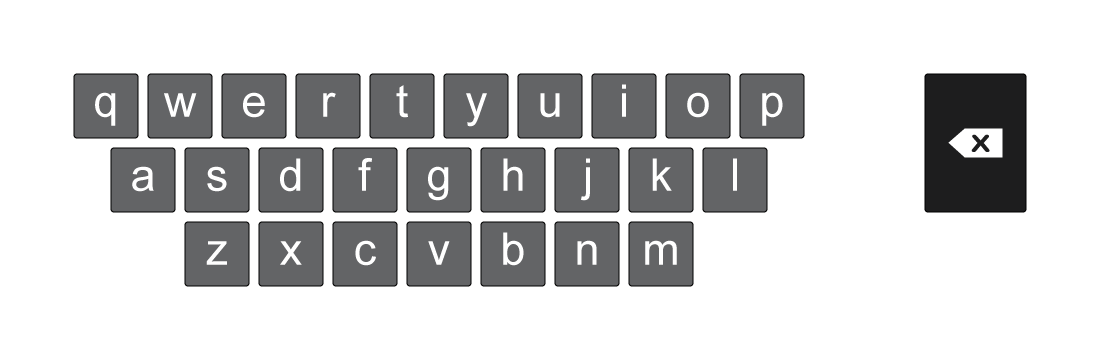
\includegraphics[width=6in]{fig_final_keyboard}
	\caption[Display: Keyboard Layout]{The keyboard layout used during the final study.}
	\label{keyboard_layout}
\end{figure}

\subsubsection{Text Area}
Figure~\ref{text_area} shows how two text areas were used to display text to participants. The top text-area showed the current word to transcribe, shown in Figure~\ref{text_a}, and the bottom area showed the currently transcribed text, shown in Figure~\ref{text_b}. The characters of both the displayed word and transcribed text were highlighted in green when the characters matched and were correct, whereas the letters in only the transcribed text would highlight in red if errors were made during transcription. The participant can then use the back space in order to correct words, and they are finally highlighted in green, as seen in Figure~\ref{text_c}, when a word was completed and correct.

\begin{figure}[h]
	\centering
	\begin{minipage}[t]{1.9in}
		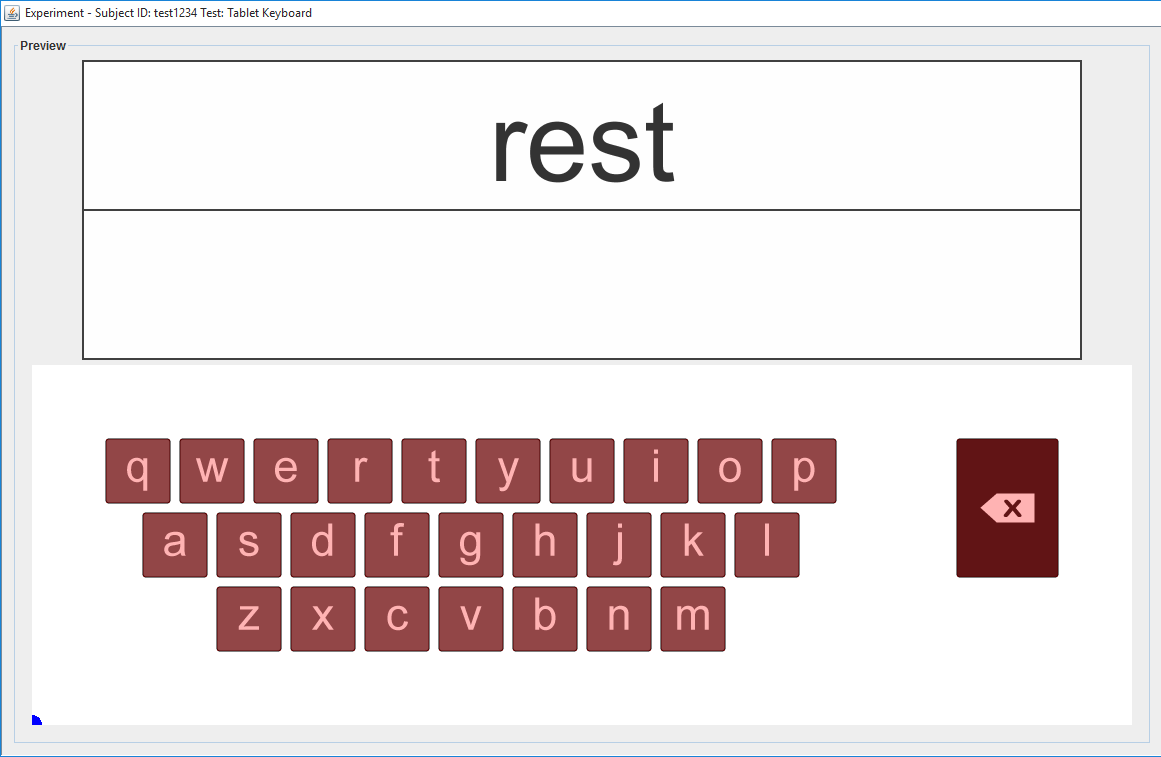
\includegraphics[width=2in]{fig_idle_keyboard}
		\subcaption{Displayed Word}
		\label{text_a}
	\end{minipage}
	\begin{minipage}[t]{1.9in}
		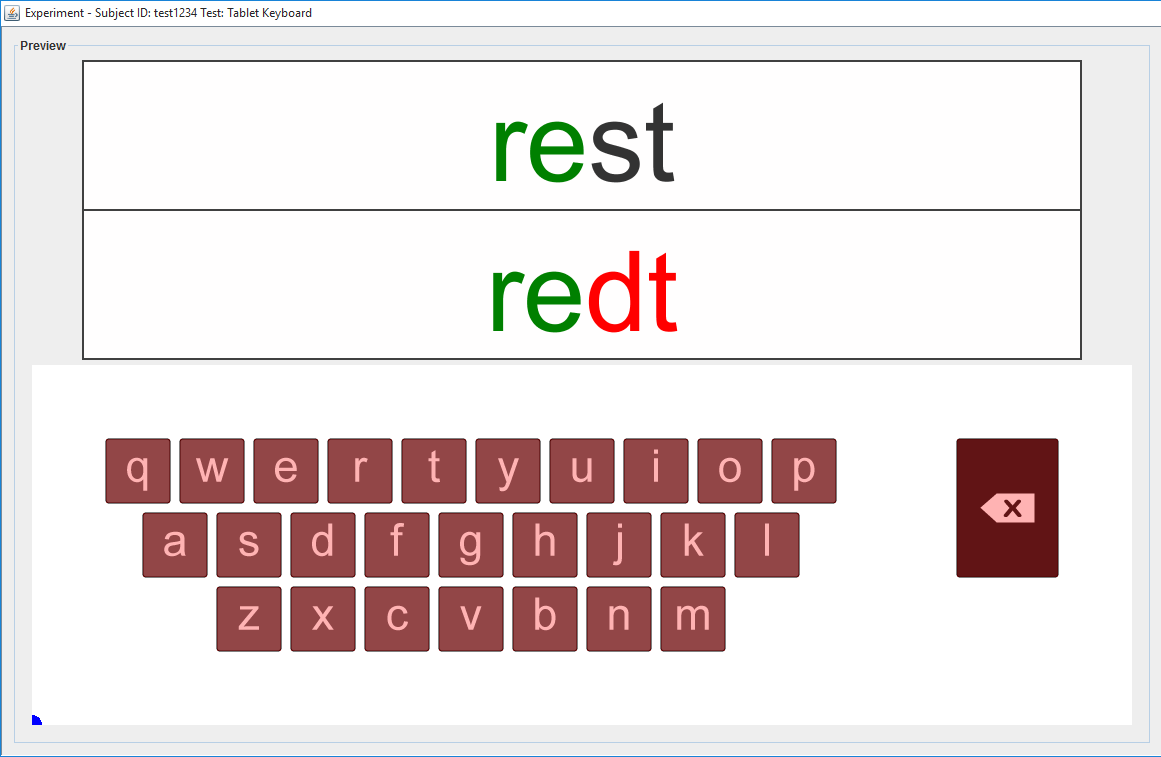
\includegraphics[width=2in]{fig_error_keyboard}
		\subcaption{Transcribed Error}
		\label{text_b}
	\end{minipage}
	\begin{minipage}[t]{1.9in}
		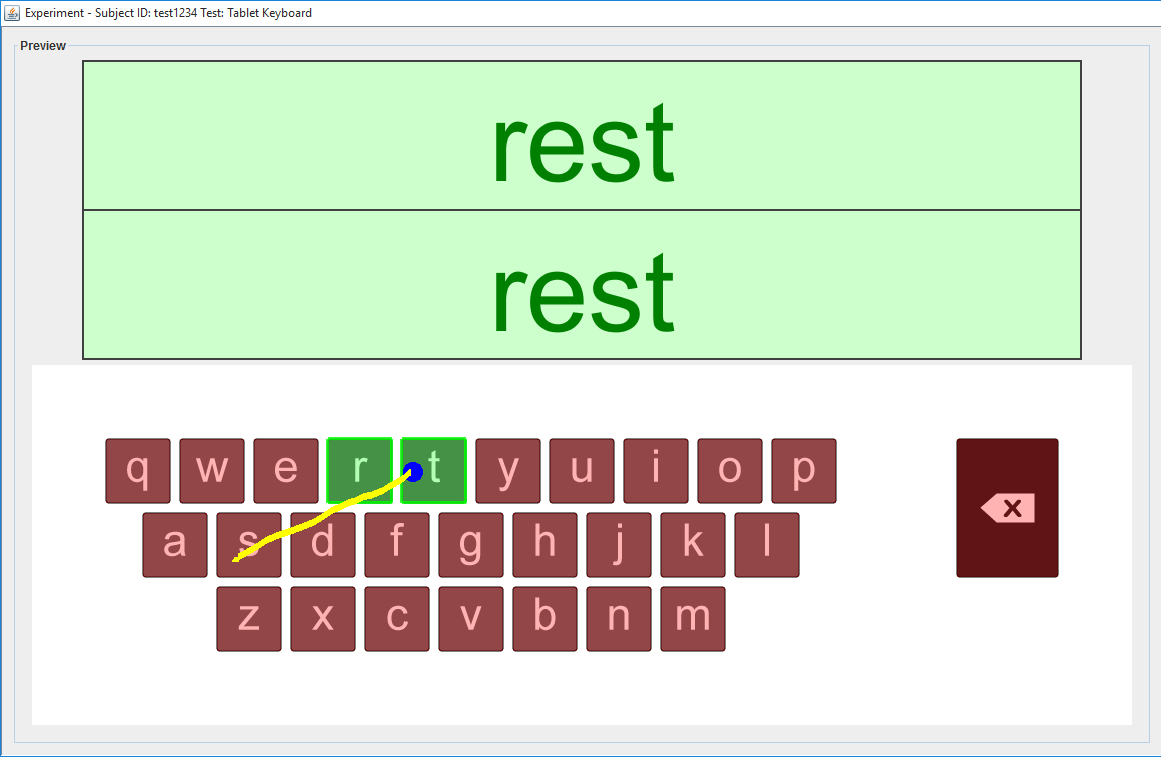
\includegraphics[width=2in]{fig_correct_keyboard}
		\subcaption{Completed Word}
		\label{text_c}
	\end{minipage}
	\caption[Display: Text Area]{Examples of how the text areas change when showing transcribed text. \textbf{(a)} shows the word to transcribe as it first appears. \textbf{(b)} shows how correct letters are highlighted green in both text areas and transcription errors are highlighted in red. \textbf{(c)} shows a completed word, the background lights up to indicate correctness.}
	\label{text_area}
\end{figure}

\subsubsection{Real-Time Updates}
As a participant is drawing the gesture-shape of a word, their progress is tracked in real time, as shown in Figure~\ref{display_area}. For the keyboards that track a participant's finger or the stylus, Figure~\ref{update_a} shows how a cylinder is displayed to indicate the direction that the finger is pointing, as well as which letter is being hovered over, indicated by a blue dot. As in Figure~\ref{update_b}, the participant is shown the path that they are traveling as well as the letter that have been hit. The gesture-trail has a maximum length before it starts to decay as to not clutter the display. 

\begin{figure}[h]
	\centering
	\begin{minipage}[t]{2.9in}
		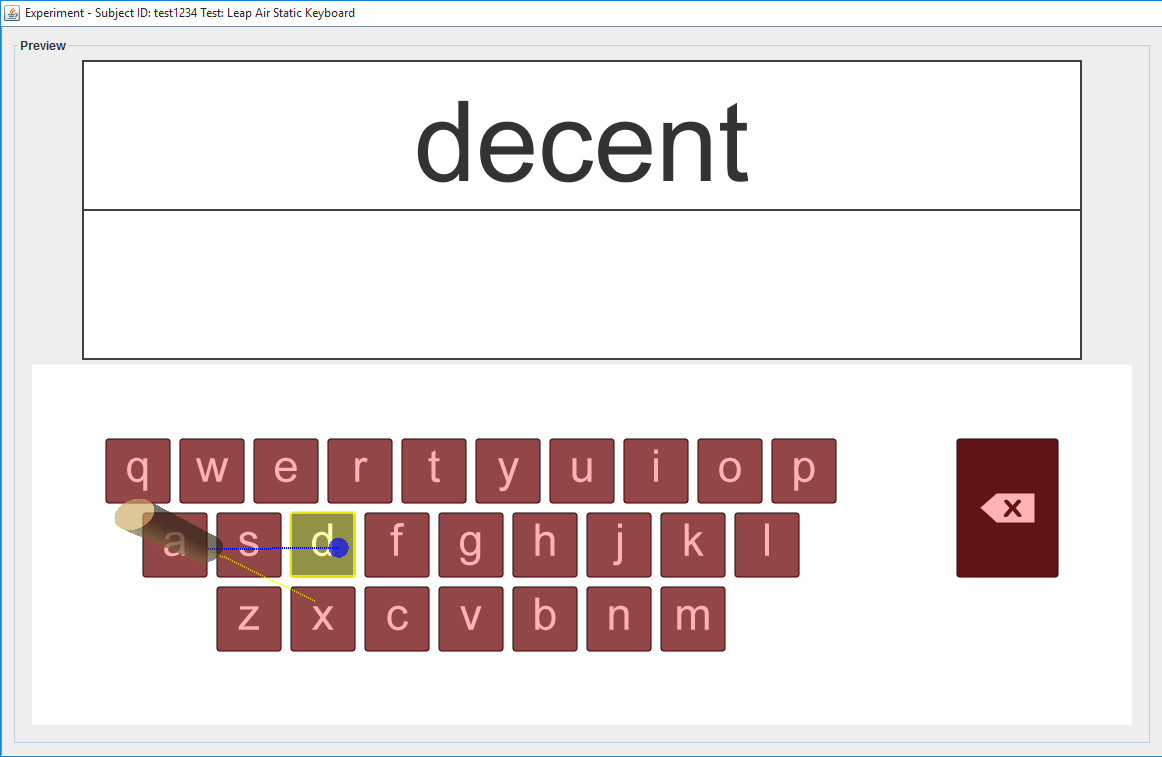
\includegraphics[width=3in]{fig_update1_keyboard}
		\subcaption{Prior to pressing 'd'}
		\label{update_a}
	\end{minipage}
	\begin{minipage}[t]{2.9in}
		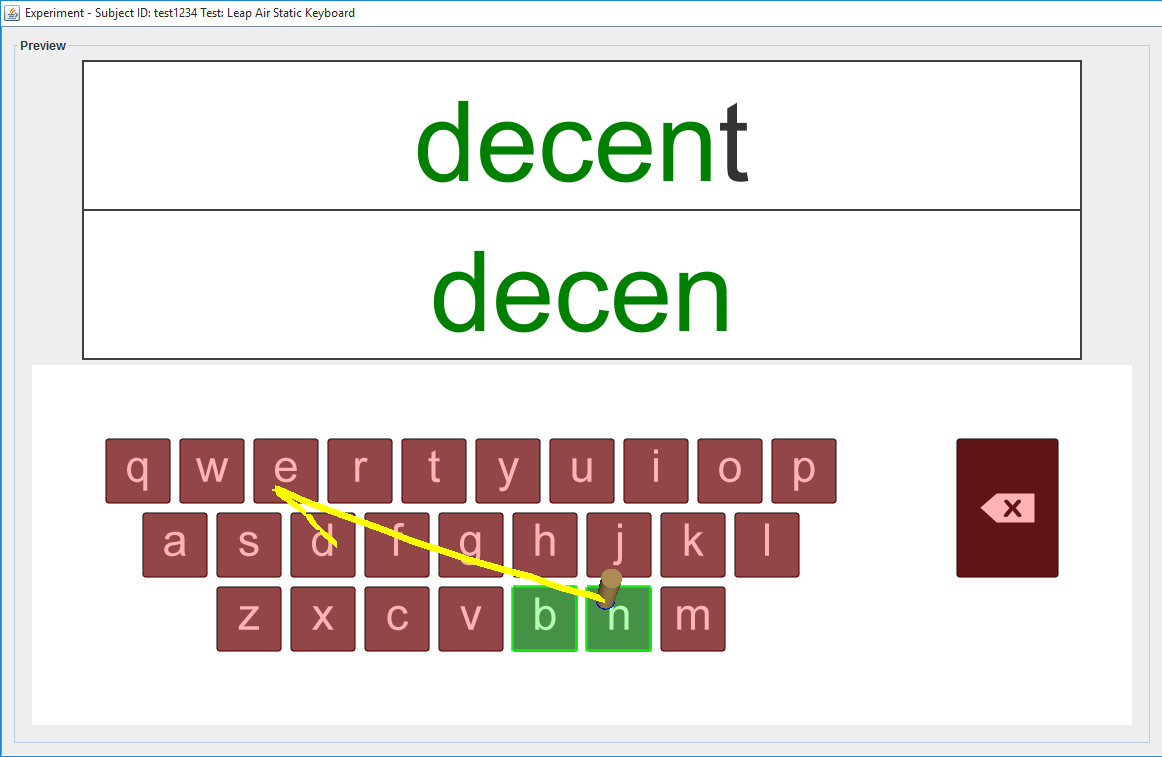
\includegraphics[width=3in]{fig_update2_keyboard}
		\subcaption{During the word-gesture}
		\label{update_b}
	\end{minipage}
	\caption[Display: Text Area]{Examples the real-time display for word-gesturing. \textbf{(a)} shows the user just about to press the first character. \textbf{(b)} shows the middle of the word gesturing process for the word "decent".}
	\label{display_area}
\end{figure}

\subsection{Dictionary Creation}
To make each keyboard experience as similar as possible, custom dictionaries were created for each keyboard input device containing words with similar gesture-shapes between keyboards. Dictionaries were created using a custom gesture-shape dissimilarity algorithm. The dictionaries contained words between the character lengths of 3 and 6 so that words would be rather simple, and words that most participants had seen before.

\subsubsection{Using Similar Gesture-Shapes}
The reason that custom dictionaries were chosen to be created was because it was thought that dependent measures would be more accurately represented for each keyboard if the experiences between those keyboards was nearly the same, only changing due to implementation. There was no previous research on words with similar gesture-shapes, or if this was truly necessary or beneficial.

\subsubsection {Gesture-Shape Dissimilarity}
Originally the Fr\'echet Distance was used to try to find the most similar word gesture-shapes using the sets of words with the least distance between each gesture-shape. Fr'echet Distance gave acceptable results, however there were noticeable differences in some of the paths created. TODO: SHOW FIGURE OF 10 WORDS FOR FRECHET vs 10 WORDS FROM MINE --- side by side comparison.

In order to achieve gesture-shapes with even closer similarity, a custom dissimilarity algorithm to rate words' gesture-shapes of the same length was created. The top results for words with the least dissimilarity between each other were then split among the dictionaries. The dissimilarity between two words is defined by the formula
\begin{equation}
dissimilarity(P,\ Q) = \frac{\sum\limits_{i = 2}^{N} \frac{1}{2} \left(\left(\frac{\mid dist(P_{i},\ P_{i-1}) - dist(Q_{i},\ Q_{i-1})\mid}{max\ distance}\right) + \left(\frac{angle(P_{i} - P_{i-1},\ Q_{i} - Q_{i-1})}{\pi}\right)\right)}{N - 1}
\end{equation}
where $P$ and $Q$ were two words of $N$ length, $P_i$ and $Q_i$ were the vector locations of the characters of the words on the virtual keyboard, $max\ distance$ was the maximum distance between any two letters on the virtual keyboard, $dist(...)$ was the distance between two vector locations, and $angle(...)$ was the angle between two vectors.

The dissimilarity formula forced values between the range [0, 1] and treated every path between two letters with equal weight. The objective was then to find the sets of words with the lowest dissimilarity

\subsection{Calibration}
Maybe mentioned gorilla arm syndrom in Chapter 2?

--- gorilla arm syndrom. Has a similar calibration as alvins Personal Space but this calibration was optional. This calibration space is also more complicated due to the nature of having to precisely interact with the generated plane.

THIS SECTION WILL GO THROUGH THE REASONS FOR CALIBRATION AND ALIVINS THING

\subsubsection{Separation of motor space and display space --- rename (figure out ordering)}

\subsubsection{Size of motor space / User calibrated --- rename (figure out ordering)}



Lack of recognition and reason for it. Simulated recognition.

\section{Word-Gesture Keyboards}

\subsection{Touch Screen Keyboard}

\subsubsection{Separating words --- rename (figure out ordering)}

\subsubsection{Size of motor space / User calibrated --- rename (figure out ordering)}




\subsection{Leap Surface Keyboard}

\subsubsection{Separating words --- rename (figure out ordering)}

\subsubsection{Size of motor space / User calibrated --- rename (figure out ordering)}




\subsection{Leap Static-Air Keyboard}

\subsubsection{Separating words --- rename (figure out ordering)}

\subsubsection{Size of motor space / User calibrated --- rename (figure out ordering)}




\subsection{Leap Predictive-Air Keyboard}

\subsubsection{Separating words --- rename (figure out ordering)}

\subsubsection{Size of motor space / User calibrated --- rename (figure out ordering)}




\subsection{Leap Bimodal-Air Keyboard}

\subsubsection{Separating words --- rename (figure out ordering)}

\subsubsection{Size of motor space / User calibrated --- rename (figure out ordering)}





\subsection{Leap Pinch-Air Keyboard}

NOTE: VULTURE PINCH FORCED AWKARD PINCH, LEAP ALLOWED FOR ANY PINCH GESTURE FOR LESS FIDELITY



\subsubsection{Separating words --- rename (figure out ordering)}

\subsubsection{Size of motor space / User calibrated --- rename (figure out ordering)}
